
\section{Especificação funcional}



Os requisitos funcionais levantados para o \it{software} são:

\begin{enumerate}[label=RF \arabic* -- , ref=\arabic*]
	\item A
	\item B
\end{enumerate}

Os requisitos não-funcionais levantados para o \it{software} são:

\begin{enumerate}[label=RNF \arabic* -- , ref=\arabic*]
	\item A
	\item B
\end{enumerate}


A Figura \ref{fig:diagrama_blocos} apresenta o diagrama de blocos com uma visão geral do sistema. Um computador executa continuamente uma simulação de elevador. O usuário interage diretamente com esta simulação através do mouse, pressionando botões (internos e externos) do elevador. O Kit LPC1768 faz o papel de controlador do elevador, gerenciando a lógica de movimentação e de abertura/fechamento de portas. O Kit e o computador comunicam-se via interface serial, sendo que o Kit controla o comportamento do elevador na simulação, e o computador envia ao Kit comandos de botões do usuário. 


\begin{figure}[h]
\begin{center}
    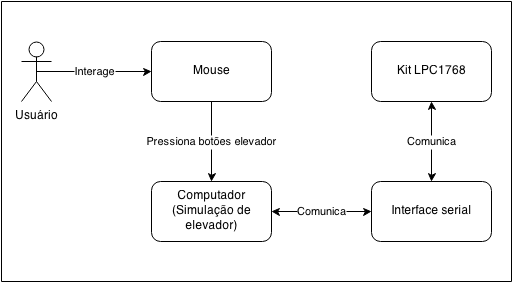
\includegraphics[width=0.8\columnwidth]{./figures/diagrama_blocos.png}
    \caption{Diagrama de blocos do sistema.}
    \label{fig:diagrama_blocos}
\end{center}
\end{figure}

